\section{Technical approach}
The main techniques for this problem can be described as follows
\begin{enumerate}
		\item \textbf{Face detection and landmark localization:} We employ dlib's face detection model, which utilizes Histogram of Oriented Gradients (HOG) features and a Support Vector Machine (SVM) classifier to locate faces in images. The system further identifies 68 facial landmarks corresponding to key facial features, establishing the foundation for emotion analysis.
		\item \textbf{Emotion classification:} We implement a Convolutional Neural Network (CNN) based on the ResNet-18 architecture to classify facial expressions into distinct emotional categories. We evaluate the model's performance against human benchmarks to validate its effectiveness, as emotion recognition is a challenging task even for humans.
\end{enumerate}
In this process, there may be some difficulties, especially in terms of efficiency. As the neural network is very computationally costly, we have to think of some methods to reduce time consumption.

The ways we thought of can be described as follows:
\subsection{Efficiency promotion}
\begin{enumerate}
    \item \textbf{Localized detection:} We know that the face can not move very fast in the picture, so we can just detect a small area around the position of faces in the last frame. We detect on the global scale only if there is no face in the last frame. You may wonder what if the scope changed suddenly, it doesn't matter. In the first frame after changing the scope, we cannot detect the face, but after that, we will find that there is no face in the last frame, and then detection on a global scale will be done. So, indeed, we may lose at most one frame, which cannot be observed.
    \item \textbf{Reduced resolution scanning:} some computation can be saved when scanning the whole picture. We can just reduce the resolution of the picture by several times, as we just need to find the position of the faces, very high resolution is not necessary. For example, we find that 480P is good enough than 1080P. The model can still find the face in 480P, and the time consumption is much less than that in 1080P.
    \item \textbf{Dynamic resolution adjustment:} when the face is very large, we can also reduce the resolution, as it is just about finding the face.
\end{enumerate}
\subsection{CNN recognition}
We observed that the data distribution was highly unbalanced, with the disgust class being significantly underrepresented while the happy class was overrepresented. To address this issue, we applied data augmentation techniques to balance the class distribution. This preprocessing step improved our classification results, particularly for the rare emotion categories that would otherwise have been difficult to recognize accurately.

We employed a ResNet architecture for emotion classification. Notably, facial expression classification is challenging even for humans. To establish a benchmark, we conducted experiments with human participants (our classmates). Initially, they achieved approximately 40\% accuracy, and even after extensive exposure to the dataset, their performance plateaued at around 65\%. Our model achieved an average test accuracy of 62\% (Figure \ref{fig:test_acc}), which is comparable to human performance on this challenging task.

\begin{figure}[!htb]
	\centering
	 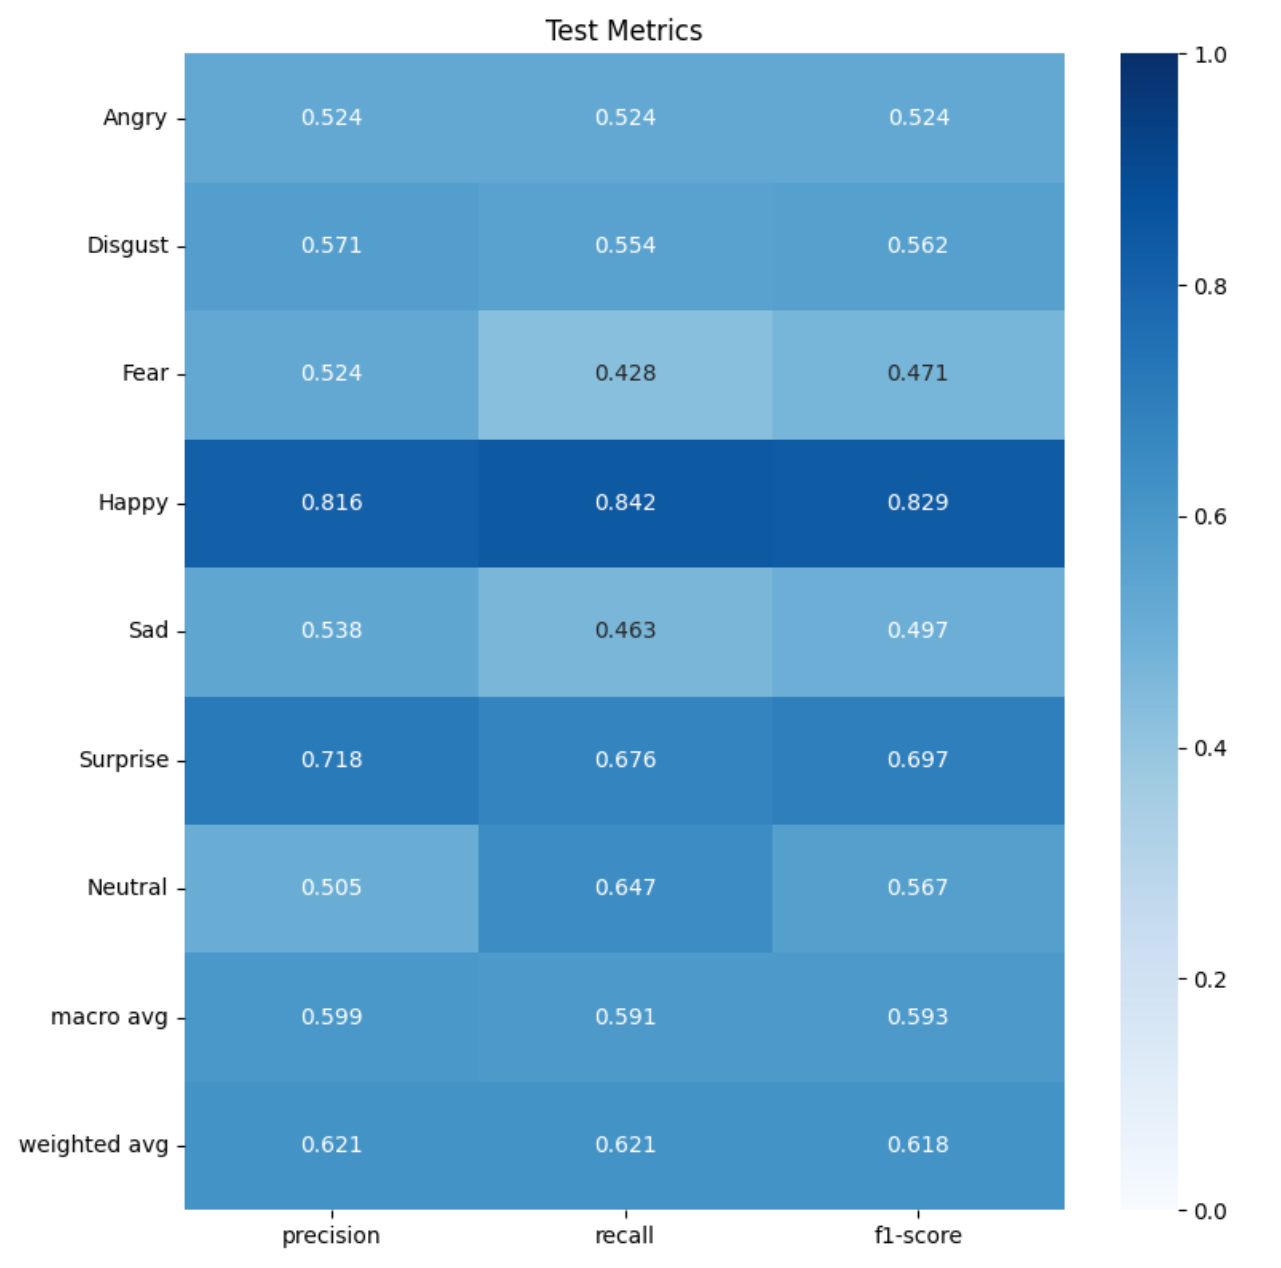
\includegraphics[width=1.0\linewidth]{sec/assets/test_acc.png}
	 \caption{The model achieved 62\% accuracy on the test set, comparable to trained human performance.}
	 \label{fig:test_acc}
\end{figure}

